\section{Results}\label{sec:results}

\noindent\emph{Status of this section.} Measured so far: the cohort description, the human annotation, the
offline verification of the pipeline, an eligibility and de-identification screen, and a single-case pilot of
Arms A and B with Gemma~4. Arm~C has not been run. Every comparative result is marked as pending and is
accompanied by the analysis that will produce it.

\subsection{Data flow}

Of the 275 de-identified summaries in the platform, 50 form the frozen cohort (\cref{fig:flow}). All
50 were planned for three independent annotations (150 assignments across six reviewers). At the data
cut of 23 September 2026, 63 annotations had been submitted by four reviewers: 7 summaries had no
submission, 24 had one, 18 had two and 1 had three. Forty-three summaries therefore have at least one
human annotation and 19 have at least two. All 50 summaries enter the structural, evidence and cost
analyses, which do not require a human reference.

\paragraph{Eligibility and de-identification screen.} The header of each summary records the units of
admission and discharge of the hospitalisation: 16 summaries started and 20 ended in the adult ICU, and the
rest started or ended in surgical, medical, intermediate-care, emergency or recovery units, which is
compatible with an ICU stay in the middle of the hospitalisation. A lexical screen found no mention of the
ICU, the high-dependency unit or intensive care in 12 of the 50 summaries; these are candidates for
exclusion from the agreement analyses, pending clinical review (Section~\ref{sec:setting}). The same screen
found the hospital record number unmasked in the header of 12 summaries, which led to the corrected
redaction and the re-export of 24 September 2026 (Section~\ref{sec:setting}); the annotation counts in this
section still refer to the 23 September cut. These counts come from a pattern search on the model
input and are reported without any identifier.

\begin{figure}[tbp]
\centering
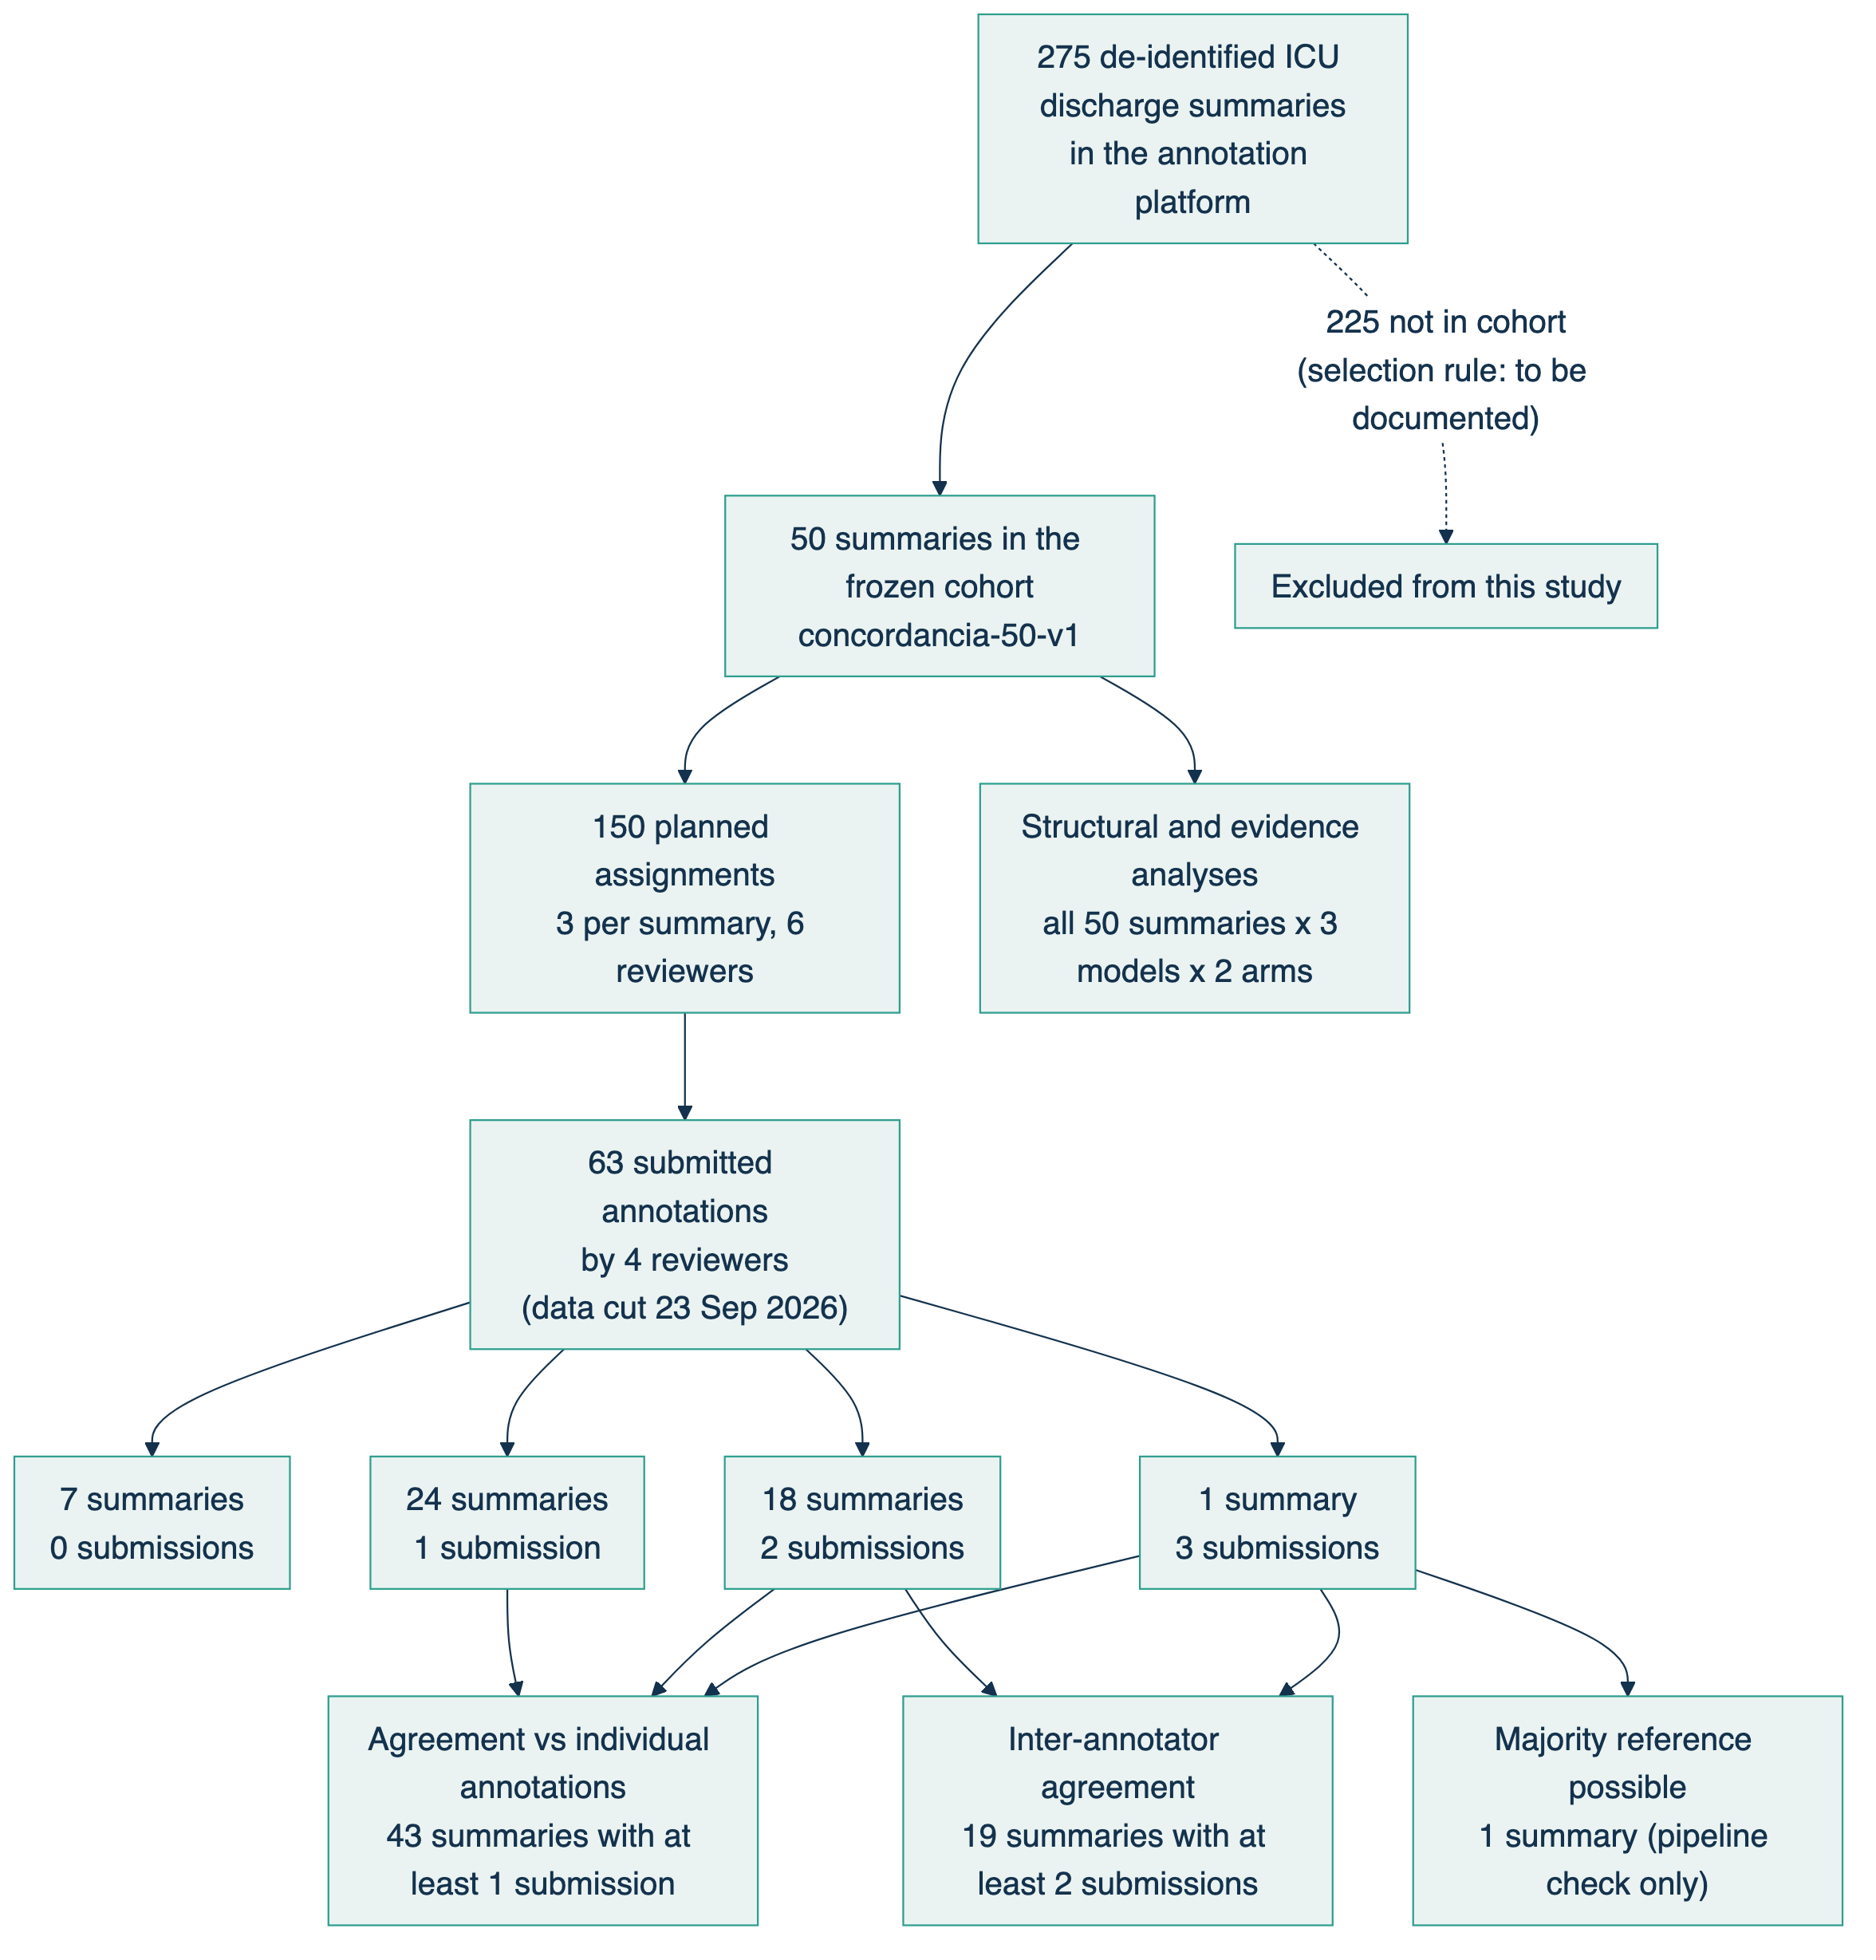
\includegraphics[width=0.78\textwidth]{figuras/png/fig3_inclusion.png}
\caption{\textbf{Inclusion and analysis sets.} Counts from the 23 September 2026 snapshot
(\texttt{snapshot.json}, \texttt{assignments.json}, \texttt{submitted\_annotations.json}). Unit: discharge
summary. Submissions are counted per summary; unsubmitted assignments are not treated as negative
annotations. The selection rule from 275 to 50 summaries is pending documentation.}
\label{fig:flow}
\end{figure}

\subsection{Cohort characteristics}

\Cref{tab:cohort} describes the cohort and the annotation workload. Summaries had a median of 3 pages
(IQR 2--3.25; range 2--6), 168.5 text spans (IQR 128--229) and 6{,}048.5 characters (IQR 3{,}270--8{,}722;
range 1{,}628--15{,}628), which yield a median of 115 indexed non-empty lines per note (range 50--303).
Clinical and demographic characteristics are not part of the model input and are not reported here
\todoauthor{decide whether aggregate age, sex, ICU length of stay and ICU mortality can be reported from
the platform's clinical data without re-identification risk}.

\begin{table}[tbp]
\centering\small
\caption{\textbf{Cohort characteristics and annotation workload.} Source:
\texttt{documents\_manifest.json}, \texttt{notes.jsonl} and the reference files of the 23 September 2026
snapshot, summarised by \texttt{scripts/cohort\_aggregates.py}. IQR, interquartile range.}
\label{tab:cohort}
\begin{tabularx}{\textwidth}{Yr}
\toprule
Characteristic & Value \\
\midrule
\multicolumn{2}{l}{\emph{Documents (unit: discharge summary, n = 50)}} \\
Pages, median (IQR) [range] & 3 (2--3.25) [2--6] \\
PDF text spans, median (IQR) [range] & 168.5 (128--229.25) [89--362] \\
Characters, median (IQR) [range] & 6{,}048.5 (3{,}270--8{,}721.75) [1{,}628--15{,}628] \\
Indexed non-empty lines, median (IQR) [range] & 115 (79.25--154.25) [50--303] \\
Total pages / spans / characters & 144 / 9{,}089 / 311{,}260 \\
\midrule
\multicolumn{2}{l}{\emph{Form}} \\
Answerable variables (boolean / date / select / text) & 199 (174 / 11 / 5 / 9) \\
Mother categories (context only, not scored) & 23 \\
Variables with a boolean ancestor / with mutual exclusions & 96 / 8 \\
\midrule
\multicolumn{2}{l}{\emph{Human annotation (data cut 23 Sep 2026)}} \\
Planned assignments (3 per summary; reviewers) & 150 (6) \\
Submitted annotations (reviewers submitting) & 63 (4) \\
Summaries with 0 / 1 / 2 / 3 submissions & 7 / 24 / 18 / 1 \\
Boolean items matched to the form: Yes / No / ? / unanswered & 1{,}189 / 9{,}729 / 0 / 43 \\
Yes answers per submission, median (IQR) [range] & 18 (10--25) [2--43] \\
Yes answers with captured evidence text & 1{,}183 of 1{,}189 \\
Boolean variables never marked Yes in any submission & 40 of 174 \\
\bottomrule
\end{tabularx}
\end{table}

\subsection{Quality of the human annotation}\label{sec:res-annotation}

Across the 63 submissions, 10{,}961 of the expected 10{,}962 boolean items could be matched to the form; in one
submission the key of one variable had been partially masked by the de-identification step during export, and that
item is excluded rather than re-mapped by hand. Of the matched items, 1{,}189 were Yes (10.8\%), 9{,}729 No and 43
left unanswered in 26 submissions. No reviewer used the ? option. Six of the 1{,}189 Yes answers lacked
captured evidence text despite the manual's requirement. Forty of the 174 boolean variables were never
marked Yes in any submission, so per-variable sensitivity and F1 are undefined for them with the current
data.

Agreement between reviewers was estimated on 19 summaries with at least two submissions, giving 21 pairs of
submissions and 3{,}616 item pairs after excluding 38 pairs with an unanswered item (\cref{tab:iaa}). Observed
agreement was 0.946 and pooled Cohen's $\kappa$ was 0.76 (95\% CI 0.70--0.82). Agreement on the presence of
a finding was lower than on its absence: positive specific agreement was 0.79 (95\% CI 0.73--0.84) and
negative specific agreement 0.97. Agreement varied by block, from $\kappa = 0.85$ for medical history to
$\kappa = 0.54$ for complications and $0.64$ for infections; the discharge block contributed only 21 item pairs.
These figures describe reviewer agreement at the data cut; they are not an estimate of model performance.
They are not directly comparable with an earlier summary produced by the platform's agreement panel on a
15 September cut (mean $\kappa$ 0.72), which averages per-criterion $\kappa$ over the 222 nodes of the form, including
mother categories, and used an earlier set of submissions.

\begin{table}[tbp]
\centering\small
\caption{\textbf{Inter-annotator agreement on the 174 boolean variables.} Unit: pair of submissions for the
same summary $\times$ variable, unanswered items excluded. $\kappa$ is Cohen's kappa pooled over item pairs;
PSA and NSA are positive and negative specific agreement. 95\% CIs from 5{,}000 case-level bootstrap
replicates (seed 20260923). Source: \texttt{datos/cohort\_aggregates.json}.}
\label{tab:iaa}
\begin{tabular}{lrrrr}
\toprule
Block & Item pairs & Observed agreement & $\kappa$ & PSA \\
\midrule
Medical history & 1{,}471 & 0.978 & 0.850 & 0.862 \\
Support and interventions & 919 & 0.940 & 0.788 & 0.824 \\
Organ failure & 186 & 0.866 & 0.711 & 0.818 \\
Infections & 874 & 0.927 & 0.642 & 0.683 \\
Complications & 145 & 0.890 & 0.537 & 0.600 \\
ICU discharge & 21 & 0.905 & 0.611 & 0.667 \\
\midrule
\makecell[l]{All boolean variables\\(19 summaries, 21 pairs)} & 3{,}616 & 0.946 & \makecell[r]{0.761\\(0.695--0.819)} & \makecell[r]{0.791\\(0.732--0.843)} \\
\bottomrule
\end{tabular}
\end{table}

\subsection{Pipeline verification}

Offline verification without inference confirmed that the generated prompts match the protocol hash, that
the catalogue contains exactly 199 unique variables in 18 groups, and that the 50 texts, the schema and the
manual match the frozen snapshot. Fifteen unit tests on synthetic notes, covering the output contract, evidence
identifiers and offsets, missingness reasons, parent--child and exclusion checks, resumption from checkpoints and
the rule that an incomplete response is never converted into No,
passed on the development machine and on the cluster within a SLURM allocation. These checks establish that
the pipeline behaves as specified on synthetic inputs; they say nothing about extraction quality.

\subsection{Pilot run}\label{sec:res-pilot}

The pilot processed the first summary of the cohort with Arms A and B and Gemma~4 under version~1.2
(\cref{tab:pilot}). On inspection, the summary described a two-day elective surgical admission without an ICU
stay, so it tests the pipeline but not the extraction of ICU variables. Both arms returned all 199 variables
with well-formed values, no truncation and valid evidence identifiers whose copied text matched the note in
every case. Arm~B needed one retry in 2 of its 18 groups; its merged output violated 6 parent--child relations,
all involving 3 non-boolean fields of invasive ventilation that one group answered as undocumented while
another group had answered that ventilation did not occur, which the protocol requires to be recorded as not
applicable. Arm~A was invalid on its first attempt (3 errors, one of them a parent--child violation within the
form) and valid after one retry. The two arms disagreed on 9 of 199 values: 4 medical-history variables and 5
ICU admission and discharge variables, which Arm~A filled from the hospitalisation while Arm~B left them empty.
Generation took 39~min in Arm~B and 3~h~47~min in Arm~A, whose single prompt of 42{,}091 tokens was decoded at
about 2 tokens per second. Earlier versions of Arm~B on the same case (versions 1 and 1.1) produced raw
responses identical to version~1.2 in all 20 calls. These observations concern one ineligible case; they are
reported as pipeline checks and carry no inferential weight.

\begin{table}[tbp]
\centering\small
\caption{\textbf{Pilot run, one summary without ICU stay, Gemma~4, version 1.2.} Source:
\texttt{datos/pilot\_v12\_gemma4.json} (aggregates without identifiers), from the traces of jobs 98635 and 98636.
Engine: Transformers with 4-bit NF4 on two RTX A6000 GPUs. No confidence intervals.}
\label{tab:pilot}
\begin{tabular}{lrr}
\toprule
 & Arm A (monolithic) & Arm B (harness) \\
\midrule
Case valid after retries & yes & no (6 relation errors) \\
Variables with a valid answer & 199/199 & 199/199 \\
Calls (retries) & 2 (1) & 20 (2) \\
Units valid at first attempt & 0/1 & 16/18 \\
Truncated calls & 0 & 0 \\
Raw responses bare / fenced / rejected & 0 / 2 / 0 & 0 / 20 / 0 \\
Input / output tokens & 93{,}939 / 25{,}485 & 104{,}648 / 14{,}831 \\
Generation time & 13{,}617 s & 2{,}331 s \\
Median output tokens per second & 1.9 & 6.4 \\
Peak GPU memory (both GPUs) & 50.2 GB & 22.1 GB \\
Boolean answers Yes / No / ? & 4 / 170 / 0 & 6 / 168 / 0 \\
Evidence items (offsets matching the note) & 14 (14) & 10 (10) \\
\bottomrule
\end{tabular}
\end{table}

\subsection{Structural validity (H1)}

\begin{resultspending}
\textbf{Table 3 (structural block).} For each model and arm: complete valid cases (/50); variable-level validity
(/9{,}950 patient--variable pairs); truncated calls and cases; omitted fields; parse outcome per call (bare, fenced, rejected) and offline
tolerant-parser sensitivity; the same outcomes on the first attempt only (sensitivity without retries); and Arm A with the
4{,}096-token budget. Differences B $-$ A with paired patient-level bootstrap 95\% CI and Holm-adjusted $p$.
\end{resultspending}

\subsection{Evidence fidelity (H2)}

\begin{resultspending}
Identifier validity (/identifiers returned), evidence coverage (/Yes and ? answers), evidence support in the
blinded review sample, and overlap with reviewer spans (/items where model and reviewer both answer Yes), by arm
and model, with paired differences and 95\% CI.
\end{resultspending}

\begin{figure}[tbp]
\begin{resultspending}[title={Figure 5 --- Evidence fidelity (RESULTS\_PENDING)}]
Grouped bars or dot plot: identifier validity, evidence coverage and evidence support, by model (panels) and arm
(colour), with 95\% CI. Denominators printed under each bar. Illustrative citation errors, if shown, must be
synthetic or fully redacted paraphrases approved by the clinical reviewers; no source text.
\end{resultspending}
\caption{Evidence fidelity by model and strategy. Source: \texttt{results/*.json} and the evidence-review form.}
\label{fig:evidence}
\end{figure}

\subsection{Agreement with human annotators (H3)}

\begin{resultspending}
\textbf{Table 3 (agreement block).} For the 174 boolean variables and each reference definition (individual,
43 summaries; concordant, 19 summaries): positive-class F1 (primary), accuracy, sensitivity, specificity,
balanced accuracy, PPV, MCC and Cohen's $\kappa$, with the model's ? handled as error and as abstention; the rate of
? per arm and model; macro-averages over variables with enough positive labels. Non-inferiority of B versus A per
model: difference in F1 with paired bootstrap 95\% CI against the margin $-\delta$.
\end{resultspending}

\begin{figure}[tbp]
\begin{resultspending}[title={Figure 4 --- Agreement by model and strategy (RESULTS\_PENDING)}]
Forest plot of positive-class F1 (point and 95\% CI) for Arm A and Arm B within each model, overall and by block,
with the difference B $-$ A and the non-inferiority margin shown as a vertical line. Unit: patient--variable pair;
resampling unit: patient; reference: individual annotations (43 summaries).
\end{resultspending}
\caption{Agreement with human annotators by model, strategy and block. Source: model results joined with
\texttt{submitted\_annotations.json} by \texttt{patient\_id} and variable key.}
\label{fig:agreement}
\end{figure}

\subsection{Cost and operational stability (H4)}

\begin{resultspending}
Per case and arm: calls, input and output tokens, latency (median, IQR), GPU-hours and peak GPU memory; retry rate
and recovery after retry; run-to-run identity in the repeatability subset.
\end{resultspending}

\begin{figure}[tbp]
\begin{resultspending}[title={Figure 6 --- Operational cost (RESULTS\_PENDING)}]
Small multiples by model: calls per case, input tokens per case, output tokens per case, latency per case and
GPU-hours for the cohort, Arm A versus Arm B, as paired dot plots (one line per case). Unit: case; denominators: 50
cases per arm and model.
\end{resultspending}
\caption{Operational cost by model and strategy. Source: inference metadata in trace files.}
\label{fig:cost}
\end{figure}

\subsection{Errors}

\begin{resultspending}
\textbf{Table 4.} Error taxonomy (\ref{app:errors}) of disagreements with the concordant reference, by arm
and model; parent--child and mutual-exclusion violations; and ablations: without retries, and Arm A with the
per-call budget. An ablation replacing evidence identifiers with model-written quotations is optional and would
require a separate pre-specified protocol version.
\end{resultspending}
